\section{Results}
\label{sec:results}
In this section, we show the outcomes of the implemented system architecture as well as the facial and vocal emotion recognition as described in Section~\ref{sec:method}.

\subsection{Experiment Environment \& Testing Setup}
\label{subsec:results_experiment_environment_and_testing_setup}
We conducted our experiments during a virtual seminar ``Collaborative Innovation Networks'' (COINs) in the summer semester of 2021 held by Prof. Peter Gloor (MIT). The seminar consisted of 23 students from the Universities of Cologne, Bamberg and Lucerne and three instructors. All students formed in total six teams with three to five participants working on complex subject-related and practical topics. Due to the global COVID-19 pandemic at that time and agile project management, all teams presented their results in weekly and bi-weekly sprints during a virtual Zoom meeting. In these virtual status meetings, every group presented their project goals, progress, results or plans of the last and next iteration and a retrospective in a short presentation of approximately ten minutes.

Since our prototype Moody was not ready for use right at the first meeting and still needed to be developed to track emotions we were only able to ask the other groups to use our Moody Tracker from the third meeting onwards. For this purpose, we wrote a short usage guide within the invitation before the meeting, so that each group could activate the tracker during their presentation. Therefore, in addition to the usage instructions, we asked the other teams to generate a feedback link via our website (\url{www.moody.digital}) after their presentation and share it with the other meeting participants.

The underlying intention here was primarily to receive instant feedback about our application in real-world usage. This made continuous testing possible, which enabled us to constantly work on errors and bugs reported by the users in each status meeting. Also, we had the chance to quickly collect subjective ratings about the perceived quality of each presentation and compare it to the tracked emotion data. The focus of this paper lies neither in statistically analyzing the correlation nor the causality between the experienced emotionality of the audience and the presentation quality, but we had the chance to cursorily analyze the first insights.

Exemplarily, Figure \ref{fig:moody_statistics_screenshot} shows a screenshot of the recorded statistics of our status presentation on the 6th July 2021. With this recording, we found that our last presenter on that day seemed to speak rather sad than happy. He was able to use this information for the next presentation to increase his positive emotion transmissions via voice. Additionally, we have seen that the faces and voices were interpreted mainly neutrally, because of the formal and informative character of the presentations. This aligns with our expectations and indicates that the models are predicting correctly.

\begin{figure}
\centering
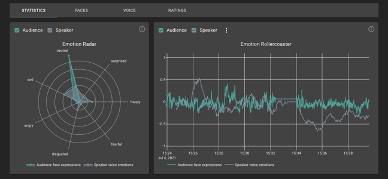
\includegraphics[width=1\textwidth]{assets/moody_statistics_screenshot.png}
\caption{Recorded statistics of the status presentation on the 6th July 2021.}
\label{fig:moody_statistics_screenshot}
\end{figure}

\subsection{Face Emotion Recognition}
\label{subsec:results_face_emotion_recognition}
Since we adopt the pre-developed \texttt{faceapi.js} and its two underlying models for face detection and expression recognition, we do not want to focus in this chapter on presenting the resulting metrics and accuracies. Instead, we briefly show that we implemented the API correctly in our tool and how it works. Figure \ref{fig:moody_faces_screenshot} illustrates the presenter's view of the detected faces and their current emotions when he clicks on the ``Faces'' tab while the emotion tracking is running. It seems that the model identifies the emotions expressed by the faces correctly.

\begin{figure}
\centering
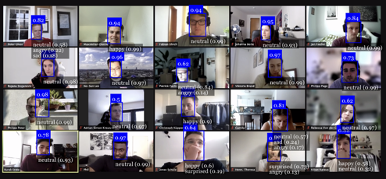
\includegraphics[width=1\textwidth]{assets/moody_faces_screenshot.png}
\caption{Presenter's view of the detected faces in the according ``Faces'' tab.}
\label{fig:moody_faces_screenshot}
\end{figure}

The models receive every second a frozen frame from the video conference window with all participants' cameras and calculate every second the probabilities for the current \citeA{ekman_universal_1997} emotion per person respectively per detected face. Thus, every emotion out of neutral, happy, sad, angry, fearful, disgusted, and surprised gets a probability between 0 and 1 assigned. Exemplarily, ``happy (0.8)'' and ``neutral (0.2)'' mean that the particular face looks 80\% happy and smiling, and is by 20\% neutrally predicted. In order to receive the overall audience emotion score to visualize in the Emotion Rollercoaster (cf. Figure \ref{fig:moody_statistics_screenshot}) we calculate the mean face emotion value from all detected faces. The emotion score lies between -1 and 1 since we assign the emotions from \citeA{ekman_universal_1997} to negative, neutral, and positive values. The probabilities for happy and surprised are assigned to 1, neutral to 0, and sad, disgusted, angry, and fearful to -1.

\subsection{Vocal Emotion Recognition}
\label{subsec:results_vocal_emotion_recognition}
Since the AlexNet was trained on the four different data sets (RAVEDESS, EMO-DB, TESS, JL-Corpus) to get as much variety as possible, the accuracy of the model is 87.17\% (cf. \nameref{app:appendix}, Figure~\ref{fig:alexnet_accuracy}). 

To get the best possible result, early stopping is included. This is best at the eighth epoch, as the loss does not change significantly afterwards (cf. \nameref{app:appendix}, Figure~\ref{fig:alexnet_loss}).

The difference to the ResNet model, apart from minor differences in accuracy, is mainly the size of the model (cf. \nameref{app:appendix}, Figures~\ref{fig:resnet_accuracy}~and~\ref{fig:resnet_loss}). The AlexNet has a size of 32.3 MB whereas the ResNet is almost twice as big with a size of 59.6 MB. Since the data model is reloaded in the browser every time the voice emotion model is used, which takes up time as well as memory, we finally decided to use the AlexNet. It has solid accuracy and smaller memory size which is ideal for usage on end-user devices. Table \ref{tab:model_comparison} depicts the model metrics in comparison.

\begin{table}
\setlength{\tabcolsep}{18pt}
\renewcommand{\arraystretch}{1.5}
\centering
\begin{tabular}{l|ll}
                       & AlexNet            & ResNet18         \\ \hline
Training accuracy      & \textbf{95.66\%}   & 91.43\%          \\
Validation accuracy    & 87.17\%            & \textbf{87.85\%} \\
Training loss          & \textbf{0.1297}    & 0.2521           \\
Validation loss        & 0.3827             & \textbf{0.3520}  \\
Best epoch             & \textbf{30}        & 35               \\
Epoch (early stopping) & 8                  & \textbf{7}       \\
Model size             & \textbf{32.3 MB}   & 59.6 MB          \\
Training duration      & \textbf{11min 17s} & 21min 51s        \\
\end{tabular}
\caption{Model metrics in comparison. The AlexNet model is used because it is more parsimonious in model size with a comparable accuracy and cross-entropy loss. Bold values are preferred.}
\label{tab:model_comparison}
\end{table}

Finally, the confusion matrix shows that our model has fairly high true prediction ratios and low deviations for almost all emotions (cf. Figure \ref{fig:alexnet_confusion_matrix}). The highest ratio of wrong predictions is for the emotion ``sad''. While the model predicts 71.19\% correctly, it predicts ``neutral'' wrongly in 20.90\% of all cases in the validation set.

\begin{figure}
\centering
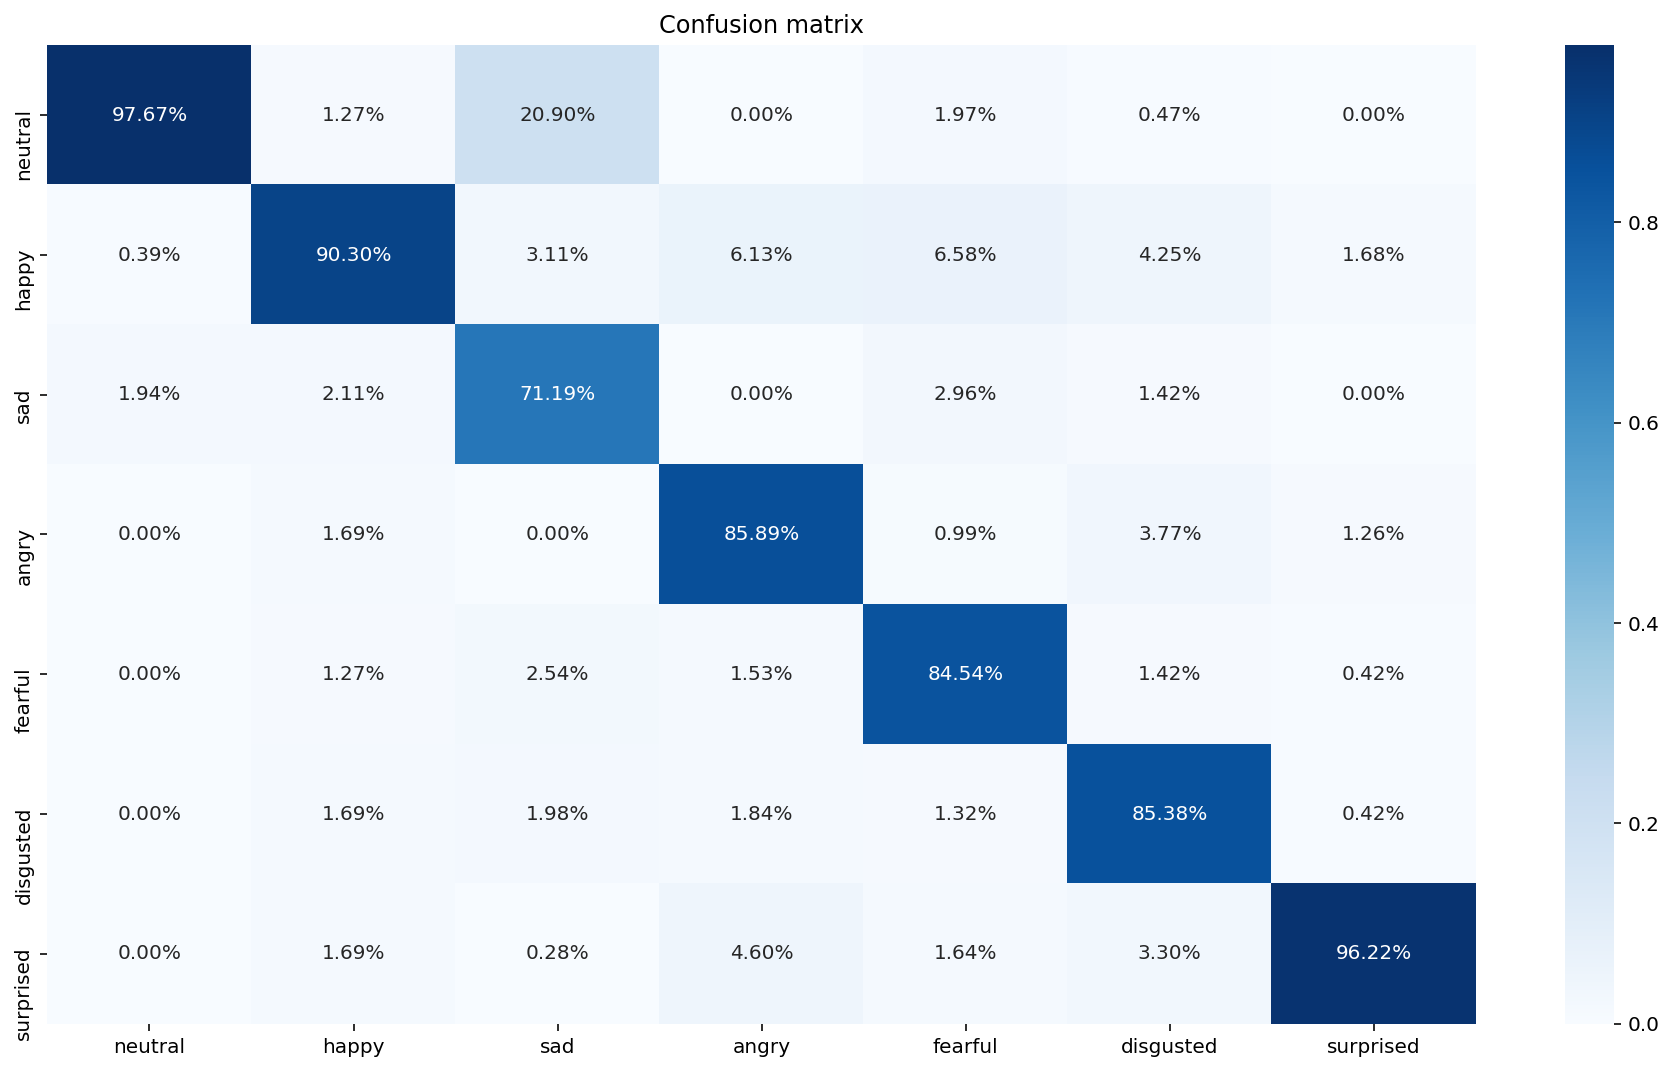
\includegraphics[width=1\textwidth]{assets/alexnet_confusion_matrix.png}
\caption{AlexNet Confusion Matrix}
\label{fig:alexnet_confusion_matrix}
\end{figure}

The voice emotion model can be activated optionally at any time during a meeting. It can be activated during the whole meeting or just at the beginning or end of the meeting and will then be downloaded by the browser in case it is not yet cached. During the meeting, in addition to the Emotion Rollercoaster, the voice emotions can also be determined in real-time. A time span of 2.1 seconds is always taken to track the current emotion, which is delivering a good prediction of the emotion at that moment.

The app calculates a moving average to make the prediction curves smoother and better readable. This way, the presenter can identify emotional trends more clearly even during longer meetings. Proper values for the moving average span are guessed in real-time by calculating $10 \cdot std(E) + log_{10}(N)$ for the $N$ tracked emotions $E$ and can be overwritten by the user after a meeting.
